\begin{figure}[ht] 
 	\centering 
 	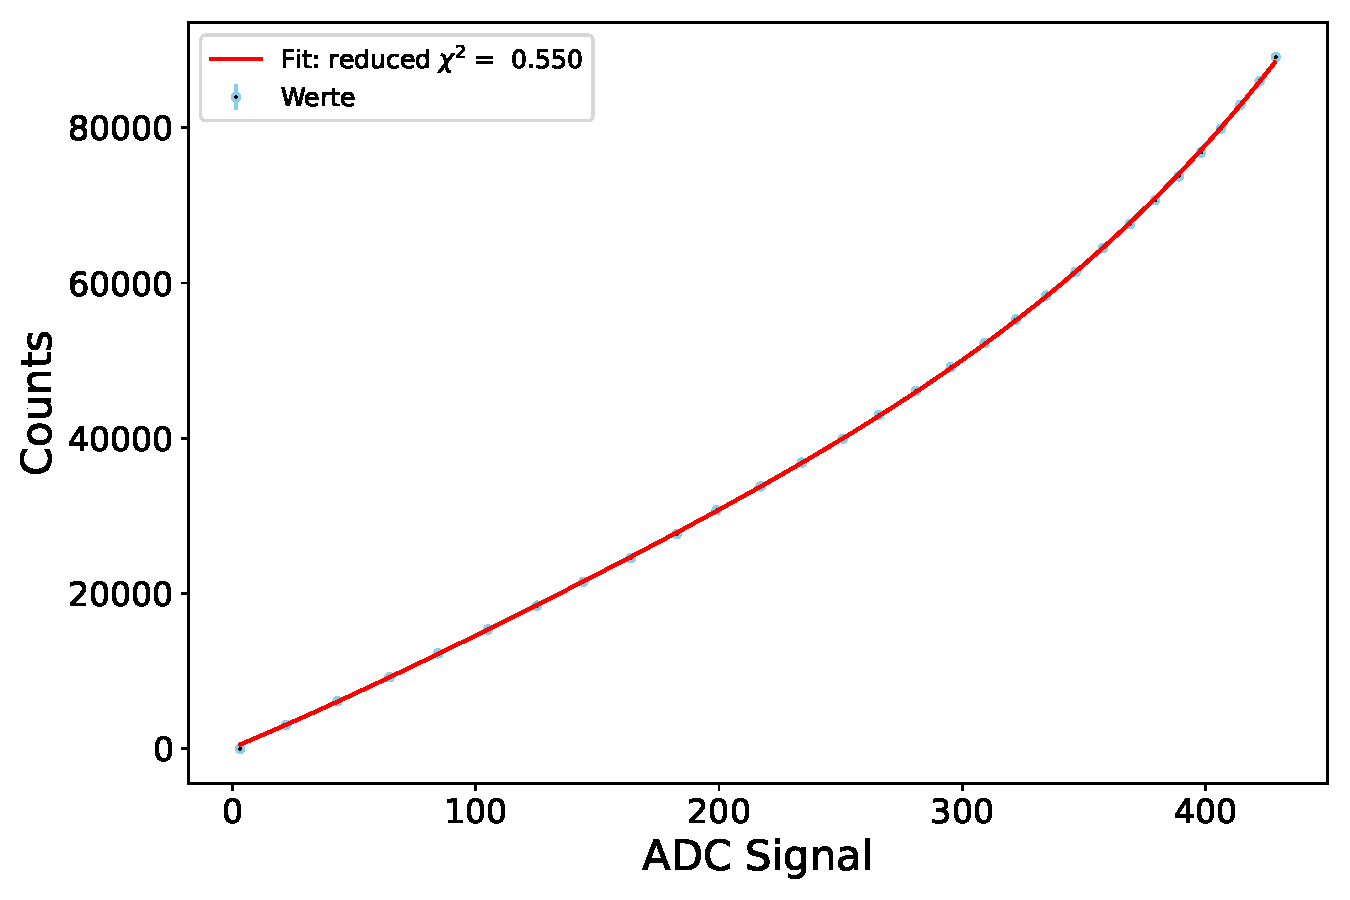
\includegraphics[width= 0.65 \textwidth]{Fits/A3_Calibration_Delay65_Fit.pdf} 
	\caption{A3_Calibration_Delay65, Fit} 
 	\label{fig:A3_Calibration_Delay65, Fit} 
\end{figure}
 \\ 
\begin{table}[ht] 
\centering 
\caption{my-table} 
\label{tab:my-table}
\begin{tabular}{|l|c|}
\hline
Parameter Name	&	Wert \\ \hline
a	&	 1.7e-06 \pm  1.5e-07\\ \hline
b	&	-0.00080555 \pm  0.000127\\ \hline
c	&	 0.211 \pm  0.0349\\ \hline
d	&	 129.791 \pm  3.448\\ \hline
e	&	 125.942 \pm  89.655\\ \hline
\end{tabular} 
\end{table}